\section{Background}
\label{background}

The World-Wide Web (WWW), commonly known as the web, was invented to allow remote collaborators to share information and ''to be a pool of human knowledge'' \parencite[76]{BernersLeeCailliauLuotonenNielsenSecret1994}. HyperText Markup Language (HTML), Cascading Style Sheets (CSS), and JavaScript (JS) are considered the core web technologies \parencite{MajchrzakBiornHansenGronli2018}. The core web technologies that are all being used today were all introduced in just a few years in 1993 to 1996 (Figure \ref{webtechnologies-timeline}).

\begin{figure}[!h]
\centering
%\fbox{
    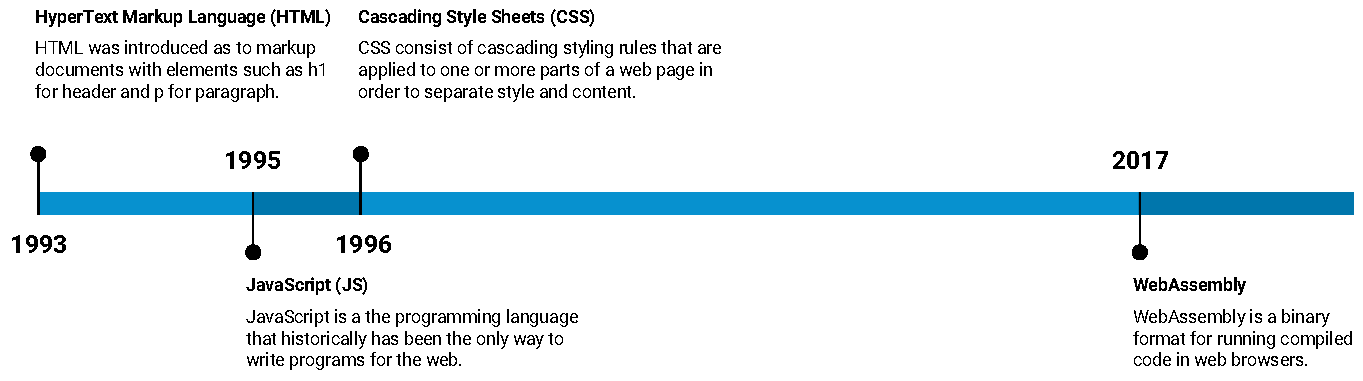
\includegraphics[width=16cm,keepaspectratio]{figures/webtechnologies-timeline}
%}
\caption{Timeline of major web technologies: HTML, CSS, JavaScript and the newest member WebAssembly.}
\label{webtechnologies-timeline}
\end{figure}

The very first web page (Figure \ref{world-wide-web}) was written in HTML and relies heavily on hyperlinks \parencite{BernersLeeCailliauGroffPollermann1992}. In 1996 the W3C recommendation on CSS was published \parencite{LieBos1996}, as a simple mechanism that ''allows authors and readers to attach style (e.g. fonts, colors and spacing) to HTML documents'' \parencite*[1]{LieBos1996} based on CSS rules. JavaScript was introduced in 1995 and was only intended to be used for simple tasks such as client-side form validation or simple animations \parencite{Moller2018}. The capabilities of JavaScript evolved and led to inventions such as Asynchronous JavaScript and XML (AJAX) \parencite{NielsonWilliamsonArlitt2008} and heavy manipulation of the Document Object Model (DOM) \parencite{WoodLeHorsApparaoByrneChampionIsaacsJacobsNicolRobieSutor1998}.

\begin{figure}[!h]
\centering
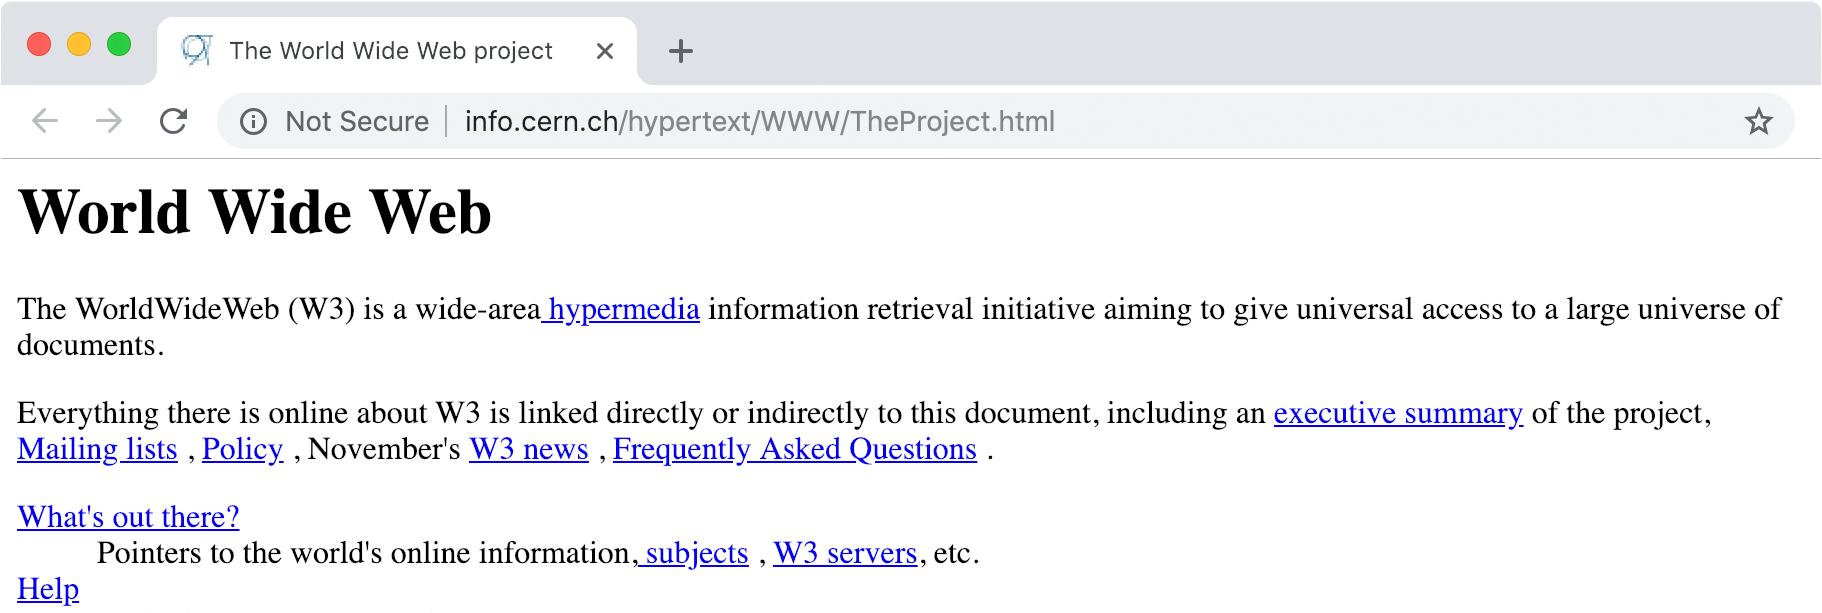
\includegraphics[width=16cm,keepaspectratio]{figures/world-wide-web}
\caption{The first web page created by Tim Berners-Lee.}
\label{world-wide-web}
\end{figure}

The introduction and evolution of JavaScript has lead the evolution of the web browser as a web page reader towards a platform for web applications.

\subsection{Web apps}
\subfile{webapps}

\subsection{JavaScript}
\subfile{javascript}

\subsection{WebAssembly}
\subfile{webassembly}
